\documentclass[letterpaper,11pt]{amsart}

\usepackage{amscd,amssymb,amsfonts,amsmath,amsthm,color}
\usepackage{enumerate}
\usepackage{listings}
\usepackage{courier}
\usepackage{graphicx}
\usepackage{scrextend}

\usepackage{calc}
\newsavebox\CBox
\newcommand\hcancel[2][0.5pt]{%
  \ifmmode\sbox\CBox{$#2$}\else\sbox\CBox{#2}\fi%
  \makebox[0pt][l]{\usebox\CBox}%  
  \rule[0.5\ht\CBox-#1/2]{\wd\CBox}{#1}}


\lstset{frame=lrbt,xleftmargin=\fboxsep,xrightmargin=-\fboxsep,colframe=gray}


\lstset{basicstyle=\ttfamily\footnotesize,breaklines=true}


%%%%%%%%%%%%%%%%%%%%%%%%%%%%%%%%%%%%%%%%%%%%%%%%%%%%%%%%%%%%
% margins and style
\pagestyle{plain}
\setlength{\evensidemargin}{0.25in}
\setlength{\oddsidemargin}{0.25in}
\setlength{\textwidth}{6.0in}
\setlength{\topmargin}{0.0in}
\setlength{\textheight}{8.5in}
\setlength{\headheight}{0in}
\setlength{\parskip}{1.5mm}

\linespread{1.2}
\usepackage{color}
\definecolor{gray}{rgb}{0.3,0.3,0.3}



%%%%%%%%%%%%%%%%%%%%%%%%%%%%%%%%%%%%%%%%%%%%%%%%%%%%%%%%%%%%
% theorems and all 
\theoremstyle{plain}
\newtheorem{theorem}{Theorem}[section]
\newtheorem{lemma}[theorem]{Lemma}
\newtheorem{proposition}[theorem]{Proposition}
\newtheorem{corollary}[theorem]{Corollary}

\theoremstyle{definition}
\newtheorem{definition}[theorem]{Definition}
\newtheorem{remark}[theorem]{Remark}

%%%%%%%%%%%%%%%%%%%%%%%%%%%%%%%%%%%%%%%%%%%%%%%%%%%%%%%%%%%%
% renewed commands: t, to, d , c, H

%%%%%%%%%%%%%%%%%%%%%%%%%%%%%%%%%%%%%%%%%%%%%%%%%%%%%%%%%%%%
% Shortcuts for tex commands

\newcommand{\nc}{\newcommand}
\newcommand{\rc}{\renewcommand}
\nc{\mc}{\mathcal}
\rc{\t}{\text}
\nc{\loccit}{\emph{loc. cit. }}
\nc\pf{\noindent Proof: }
%%%%%%%%%%%%%%%%%%%%%%%%%%%%%%%%%%%%%%%%%%%%%%%%%%%%%%%%%%%%
% Operators, functions etc
\nc{\Hom}{\t{Hom}}
\nc{\tot}{\t{tot}}
\nc{\dual}{^{\vee}}
\nc{\op}[1]{\operatorname{#1}}
\nc{\coh}{\t{coh}}
\nc{\iso}{\cong}
\rc{\d}{\operatorname{d}}
\nc{\Id}{\operatorname{Id}}
\nc{\dgmod}{\operatorname{dg-mod}}
\newcommand{\hdot}{^{\raisebox{0pt}{\text{\circle*{2}}}}}
\nc{\compose}{\circ}
\nc{\sheafsym}{\mathcal{S}\t{ym}}
\nc{\rend}{\operatorname{REnd}}
\nc{\rhom}{\operatorname{RHom}}
\nc{\sheafrend}{\mathcal{R}\mc{E}\t{\emph{nd}}}
\nc{\sheafrhom}{\mathcal{R}\mc{H}\t{\emph{om}}}
\nc{\sheafhom}{\mathcal{H}\t{om}}
\nc{\exterior}{{\textstyle\bigwedge\nolimits}}
\nc{\ex}{\exterior}
\nc{\cok}{\operatorname{Coker}}
\rc{\ker}{\operatorname{Ker}}
\nc{\im}{\operatorname{Im}}

%tensor product
\nc{\Lotimes}{{\overset{L}{\otimes}}}
%%%%%%%%%%%%%%%%%%%%%%%%%%%%%%%%%%%%%%%%%%%%%%%%%%%%%%%%%%%%
% Arrows and signs
\rc{\to}{\rightarrow}
\nc{\ot}{\leftarrow}
\nc\xto[1]{\xrightarrow{#1}}
\nc{\too}{\longrightarrow}
\nc{\oot}{\longleftarrow}
\nc{\into}{\hookrightarrow}
\nc{\mapsinto}{\hookrightarrow}
%%%%%%%%%%%%%%%%%%%%%%%%%%%%%%%%%%%%%%%%%%%%%%%%%%%%%%%%%%%%
% Categories
\nc{\D}{\operatorname{D}}
\nc{\Dsg}{\D_{{sg}}}
\nc{\Db}{\D^{{b}}}
\nc{\Dbgr}{\Db_{{gr}}}
\nc{\Dgr}{\D_{{gr}}}
\nc{\Dsggr}{\Dsg^{{gr}}}
\nc{\Cgr}{\operatorname{C}_{{gr}}}
\nc{\cCgr}{\cC_{gr}}
\nc{\cDgr}{\cD_{gr}}
\nc{\cDsggr}{\cD_{gr}^{sg}}
\nc{\cDbgr}{\cD_{gr}^{b}}
\nc{\cDsg}{\cD_{sg}}
\nc{\cDb}{\cD^{b}}
\rc{\H}{\operatorname{H}}

%%%%%%%%%%%%%%%%%%%%%%%%%%%%%%%%%%%%%%%%%%%%%%%%%%%%%%%%%%%%
% Nice letters
% cals
\nc{\cA}{\mc{A}}\nc{\cB}{\mc{B}}\nc{\cC}{\mc{C}}\nc{\cD}{\mc{D}}\nc{\cE}{\mc{E}}\nc{\cF}{\mc{F}}\nc{\cG}{\mc{G}}\nc{\cH}{\mc{H}}\nc{\cI}{\mc{I}}\nc{\cJ}{\mc{J}}\nc{\cK}{\mc{K}}\nc{\cL}{\mc{L}}\nc{\cM}{\mc{M}}\nc{\cN}{\mc{N}}\nc{\cO}{\mc{O}}\nc{\cP}{\mc{P}}\nc{\cQ}{\mc{Q}}\nc{\cR}{\mc{R}}\nc{\cS}{\mc{S}}\nc{\cT}{\mc{T}}\nc{\cU}{\mc{U}}\nc{\cV}{\mc{V}}\nc{\cW}{\mc{W}}\nc{\cX}{\mc{X}}\nc{\cY}{\mc{Y}}\nc{\cZ}{\mc{Z}}
% bbs
\nc{\PP}{\mathbb{P}}
\nc{\CC}{\mathbb{C}}
\nc{\ZZ}{\mathbb{Z}}
\nc{\HH}{\mathbb{H}}
\nc{\NN}{\mathbb{N}}
\nc{\QQ}{\mathbb{Q}}
\nc{\RR}{\mathbb{R}}


\nc{\code}[1]{{\texttt{#1}}}
\nc{\mcode}[1]{{\text{\texttt{#1}}}}



%%%%%%%%%%%%%%%%%%%%%%%%%%%%%%%%%%%%%%%%%%%%%%%%%%%%%%%%%%%%
% other useful commands
\let\oldmarginpar\marginpar
\renewcommand\marginpar[1]{\-\oldmarginpar[\raggedleft\footnotesize #1]%
{\raggedright\footnotesize #1}}
\nc\note[1]{\marginpar{#1}}

%%%%%%%%%%%%%%%%%%%%%%%%%%%%%%%%%%%%%%%%%%%%%%%%%%%%%%%%%%%%
%%%%%%%%%%%%%%%%%%%%%%%%%%%%%%%%%%%%%%%%%%%%%%%%%%%%%%%%%%%%
%%%%%%%%%%%%%%%%%%%%%%%%%%%%%%%%%%%%%%%%%%%%%%%%%%%%%%%%%%%%
%%%%%%%%%%%%%%%%%%%%%%%%%%%%%%%%%%%%%%%%%%%%%%%%%%%%%%%%%%%%
%%%%%%%%%%%%%%%%%%%%%%%%%%%%%%%%%%%%%%%%%%%%%%%%%%%%%%%%%%%%

\title{Homework 4}
\date{}
\begin{document}
\maketitle
\begin{center}
  \emph{Due Thursday, Feb 9, at 11pm}
  \vspace{0.3in}
  \end{center}


\noindent Please enter your answers into a Jupyter notebook and submit by the deadline via canvas.

\subsection*{Problem 1} Write a function \code{to\_binary(n)} that will return the binary representation of an integer. E.g. \code{to\_binary(13)} should return \code{1101}. Write a function \code{from\_binary(n)} that will return the base 10 representation of a binary number. e.g. \code{from\_binary(1101)} shoul return \code{13}. These two functions should be inverses of each other.  

\subsection*{Problem 2} Goldbach's conjecture.

The famous Goldbach conjecture states that every even number $n>2$ is a sum of two prime numbers. For example: $4 = 2 + 2$, $6 = 3 + 3$, $8 = 5 + 3$, $10 = 7 + 3$, $12 = 7 + 5$,\dots

Write Python code that checks Goldbach's conjecture for $n$ up to 10000. Print out how the even numbers from $9900$ to $9998$ can be written as sums of prime numbers. (feel free to use your \code{primes(n)}, which returned a list of primes up to n from the previous assignment to save time)


\subsection*{Problem 4} Recursion problems. Here is an example of a recursive function: (if you understand how this works, you understand recursion)

\begin{lstlisting}[language=Python]
# returns the reverse of the list xs
def reverso(xs):
    if xs == []:
        return xs
    return xs[-1:]+reverso(xs[:-1])
\end{lstlisting}

Write the following functions only using recursion. (Please don't use loops, the idea is for us to learn to use recursion. If I gave you only recursion exercises that are easier to do with recursion and hard to do with loops, they would be very difficult and it would make it much harder for you to learn to use recursion. Also don't use the built-in function \code{max} for solving \code{max} etc.)


\begin{enumerate}
  \item \code{maximo(xs)}, returns the maximum of a list of numbers. 
  \item \code{lengtho(xs)}, returns the length of a list. 
  \item \code{ispalin(xs)} returns True if xs is a palindrome (a palindrom is a sequnce that is the same in reverse, example: ``amanaplanacanalpanama''). 
  %\item \code{alternating(n)} returns a list  \code{[1,-2,3,-4,\dots,n-1,-n]} (last element + or - depending on parity). hint: 
%\begin{lstlisting}
%def f(n, sign):
  %... call f but with sign variable switched between 1 & -1, this way you are keeping track of the functions between the calls. and build the list you want with what f returns
%def alternating(n):
  %return f(n,1)
%\end{lstlisting}
  %\item \code{reverso2(xs)}, reverses a list xs. (the reverso we wrote abve returned the reverse but didn't reverse xs if it already existed, this function will reverse the list but won't return anything)
  \item \code{gcd(a,b)}, returns the greatest common divisor of two integers \code{a} and \code{b}. Use Euclid's algorithm, but implement it using recursion. Look at the notes from lecture 6 to remember (key fact: if \code{a = b*q + r}, then \code{gcd(a,b) = gcd(b,r)}).
  
\end{enumerate}

\subsection*{Problem 5} Make the following picture by modifying the code below. (use recursion, you will need the python file libhw01.py that came with the first homework) 

\begin{center}
\noindent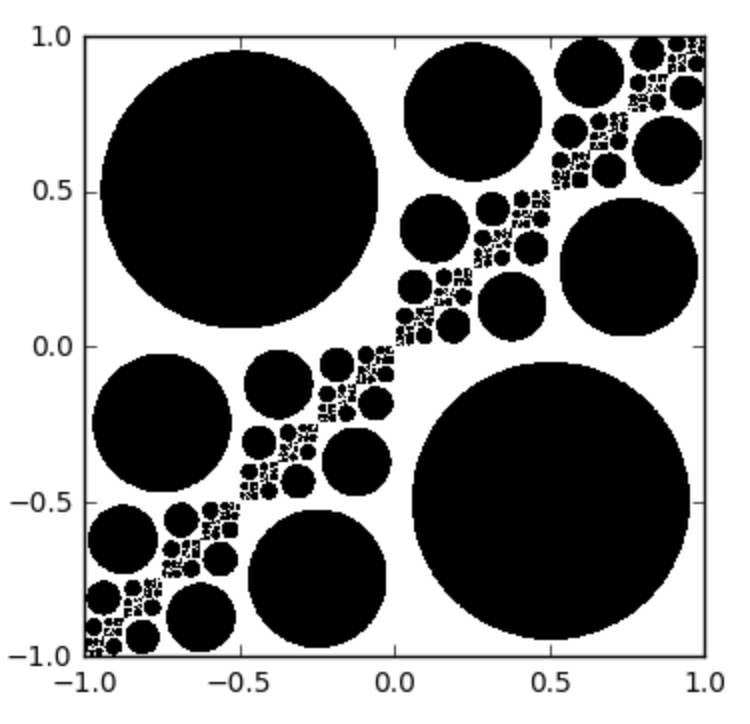
\includegraphics[width=2.9in]{fractaa.png}
\end{center}
\begin{lstlisting}[language=python]
import libhw01 as libhw

def circ(x,y):
    return 0.0 if x*x + y*y < 0.8 else 1.0

def f(x,y,count):
    # if, when you call f recursively you use f(?,?,count+1), then the count variable will keep track of how many times f called itself (how deep you are in the recursion tree if you like) and will stop calling itself indefinitely for bad values
    if count > 500: 
        return 1.0
    
    if . . .
    
def g(x,y):
    return f(x,y,0)

libhw.drawfunction(g)
\end{lstlisting}


\newpage

\end{document}
%%%%%%%%%%%%%%%%%%%%%%%%%%%%%%%%%%%%%%%%%%%%%%%%%%%%%%%%%%%%








